\documentclass{standalone}
\usepackage{tikz}
\usetikzlibrary{patterns, positioning}


\begin{document}
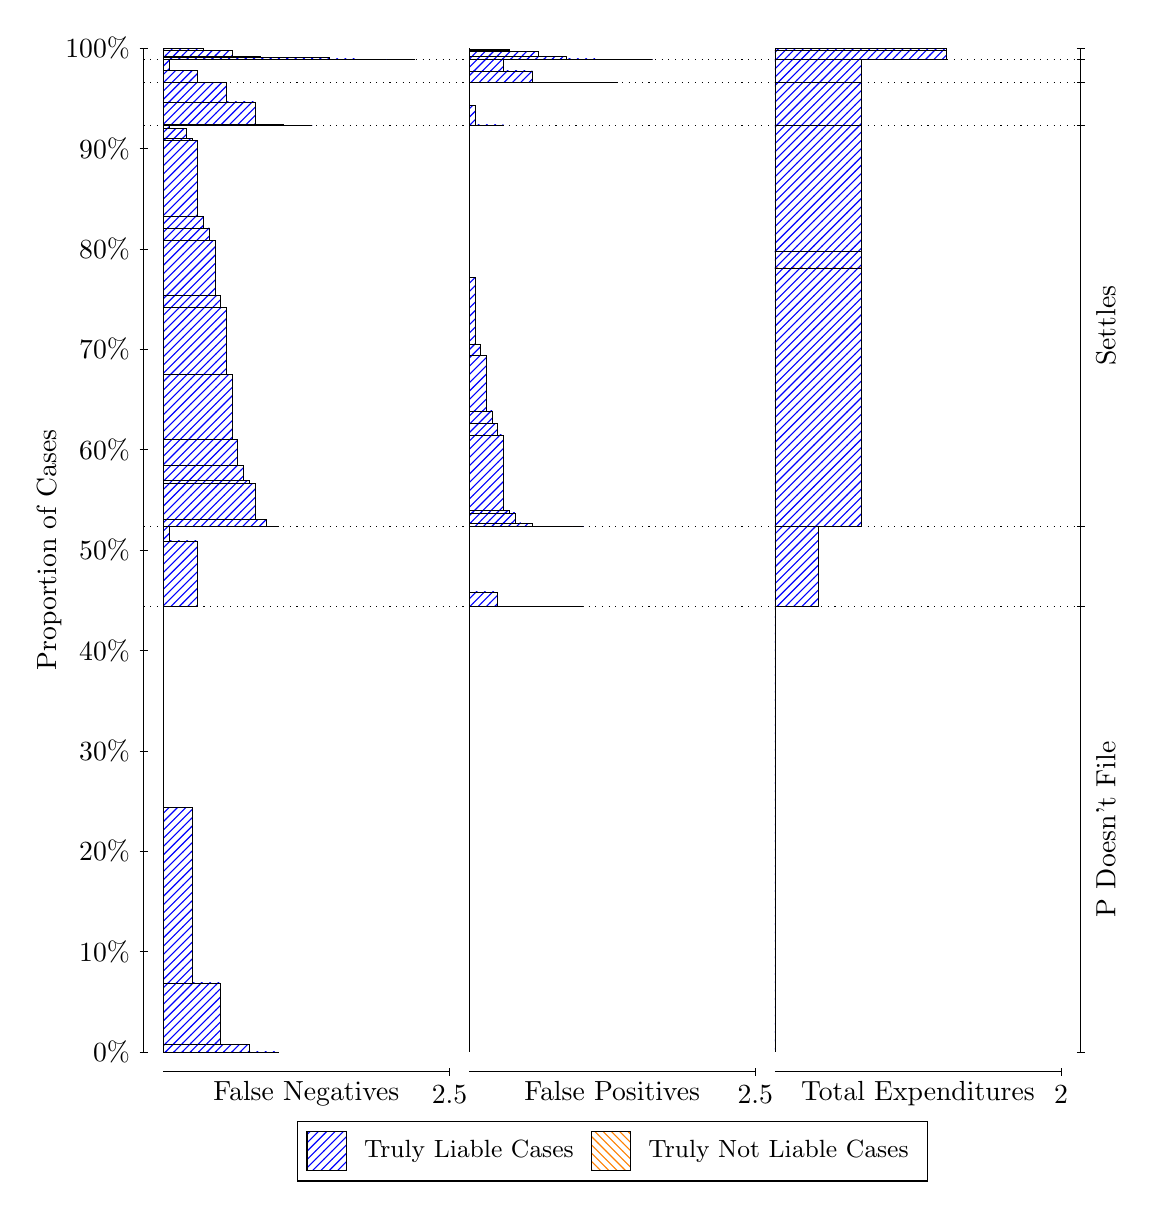
\begin{tikzpicture}
\draw[black, very thin] (1.5,1.75) -- (1.5,14.5);
\node[rotate=90, text=black, anchor=center] at (0.3, 8.125) {Proportion of Cases};
\draw[black, very thin] (1.45,1.75) -- (1.55,1.75);
\node[text=black, anchor=east] at (1.45, 1.75) {0\%};
\draw[black, very thin] (1.45,3.025) -- (1.55,3.025);
\node[text=black, anchor=east] at (1.45, 3.025) {10\%};
\draw[black, very thin] (1.45,4.3) -- (1.55,4.3);
\node[text=black, anchor=east] at (1.45, 4.3) {20\%};
\draw[black, very thin] (1.45,5.575) -- (1.55,5.575);
\node[text=black, anchor=east] at (1.45, 5.575) {30\%};
\draw[black, very thin] (1.45,6.85) -- (1.55,6.85);
\node[text=black, anchor=east] at (1.45, 6.85) {40\%};
\draw[black, very thin] (1.45,8.125) -- (1.55,8.125);
\node[text=black, anchor=east] at (1.45, 8.125) {50\%};
\draw[black, very thin] (1.45,9.4) -- (1.55,9.4);
\node[text=black, anchor=east] at (1.45, 9.4) {60\%};
\draw[black, very thin] (1.45,10.675) -- (1.55,10.675);
\node[text=black, anchor=east] at (1.45, 10.675) {70\%};
\draw[black, very thin] (1.45,11.95) -- (1.55,11.95);
\node[text=black, anchor=east] at (1.45, 11.95) {80\%};
\draw[black, very thin] (1.45,13.225) -- (1.55,13.225);
\node[text=black, anchor=east] at (1.45, 13.225) {90\%};
\draw[black, very thin] (1.45,14.5) -- (1.55,14.5);
\node[text=black, anchor=east] at (1.45, 14.5) {100\%};

\draw[black, very thin] (13.4,1.75) -- (13.4,14.5);
\draw[black, very thin] (13.35,1.75) -- (13.45,1.75);
\node[anchor=west] at (13.35, 1.75) {};
\draw[black, very thin] (13.35,7.4073) -- (13.45,7.4073);
\node[anchor=west] at (13.35, 7.4073) {};
\draw[black, very thin] (13.35,8.4266) -- (13.45,8.4266);
\node[anchor=west] at (13.35, 8.4266) {};
\draw[black, very thin] (13.35,13.52) -- (13.45,13.52);
\node[anchor=west] at (13.35, 13.52) {};
\draw[black, very thin] (13.35,14.064) -- (13.45,14.064);
\node[anchor=west] at (13.35, 14.064) {};
\draw[black, very thin] (13.35,14.359) -- (13.45,14.359);
\node[anchor=west] at (13.35, 14.359) {};
\draw[black, very thin] (13.35,14.5) -- (13.45,14.5);
\node[anchor=west] at (13.35, 14.5) {};

\draw[black, very thin, pattern color=blue, pattern=north east lines] (1.75,1.75) rectangle (3.2033,1.7509);
\draw[black, very thin, pattern color=blue, pattern=north east lines] (1.75,1.7509) rectangle (2.84,1.8422);
\draw[black, very thin, pattern color=blue, pattern=north east lines] (1.75,1.8422) rectangle (2.4767,2.6277);
\draw[black, very thin, pattern color=blue, pattern=north east lines] (1.75,2.6277) rectangle (2.1133,4.8605);
\draw[black, very thin, pattern color=orange, pattern=north west lines] (1.75,4.8605) rectangle (1.75,4.8605);
\draw[black, very thin, pattern color=blue, pattern=north east lines] (1.75,4.8605) rectangle (1.75,7.4073);
\draw[black, very thin, pattern color=blue, pattern=north east lines] (1.75,7.4073) rectangle (2.186,8.2421);
\draw[black, very thin, pattern color=blue, pattern=north east lines] (1.75,8.2421) rectangle (1.8227,8.4216);
\draw[black, very thin, pattern color=orange, pattern=north west lines] (1.75,8.4216) rectangle (1.75,8.4216);
\draw[black, very thin, pattern color=blue, pattern=north east lines] (1.75,8.4216) rectangle (1.75,8.4266);
\draw[black, very thin, pattern color=blue, pattern=north east lines] (1.75,8.4266) rectangle (3.2033,8.4267);
\draw[black, very thin, pattern color=blue, pattern=north east lines] (1.75,8.4267) rectangle (3.058,8.5148);
\draw[black, very thin, pattern color=blue, pattern=north east lines] (1.75,8.5148) rectangle (2.9127,8.9701);
\draw[black, very thin, pattern color=blue, pattern=north east lines] (1.75,8.9701) rectangle (2.84,9.0075);
\draw[black, very thin, pattern color=blue, pattern=north east lines] (1.75,9.0075) rectangle (2.7673,9.1957);
\draw[black, very thin, pattern color=blue, pattern=north east lines] (1.75,9.1957) rectangle (2.6947,9.5281);
\draw[black, very thin, pattern color=blue, pattern=north east lines] (1.75,9.5281) rectangle (2.622,10.358);
\draw[black, very thin, pattern color=blue, pattern=north east lines] (1.75,10.358) rectangle (2.5493,11.209);
\draw[black, very thin, pattern color=blue, pattern=north east lines] (1.75,11.209) rectangle (2.4767,11.355);
\draw[black, very thin, pattern color=blue, pattern=north east lines] (1.75,11.355) rectangle (2.404,12.055);
\draw[black, very thin, pattern color=blue, pattern=north east lines] (1.75,12.055) rectangle (2.3313,12.215);
\draw[black, very thin, pattern color=blue, pattern=north east lines] (1.75,12.215) rectangle (2.2587,12.361);
\draw[black, very thin, pattern color=blue, pattern=north east lines] (1.75,12.361) rectangle (2.186,13.323);
\draw[black, very thin, pattern color=blue, pattern=north east lines] (1.75,13.323) rectangle (2.1133,13.351);
\draw[black, very thin, pattern color=blue, pattern=north east lines] (1.75,13.351) rectangle (2.0407,13.478);
\draw[black, very thin, pattern color=blue, pattern=north east lines] (1.75,13.478) rectangle (1.968,13.483);
\draw[black, very thin, pattern color=blue, pattern=north east lines] (1.75,13.483) rectangle (1.8953,13.484);
\draw[black, very thin, pattern color=blue, pattern=north east lines] (1.75,13.484) rectangle (1.8227,13.52);
\draw[black, very thin, pattern color=orange, pattern=north west lines] (1.75,13.52) rectangle (1.75,13.52);
\draw[black, very thin, pattern color=blue, pattern=north east lines] (1.75,13.52) rectangle (1.75,13.52);
\draw[black, very thin, pattern color=blue, pattern=north east lines] (1.75,13.52) rectangle (3.6393,13.52);
\draw[black, very thin, pattern color=blue, pattern=north east lines] (1.75,13.52) rectangle (3.276,13.53);
\draw[black, very thin, pattern color=blue, pattern=north east lines] (1.75,13.53) rectangle (2.9127,13.815);
\draw[black, very thin, pattern color=blue, pattern=north east lines] (1.75,13.815) rectangle (2.5493,14.061);
\draw[black, very thin, pattern color=blue, pattern=north east lines] (1.75,14.061) rectangle (2.186,14.064);
\draw[black, very thin, pattern color=orange, pattern=north west lines] (1.75,14.064) rectangle (1.75,14.064);
\draw[black, very thin, pattern color=blue, pattern=north east lines] (1.75,14.064) rectangle (2.186,14.215);
\draw[black, very thin, pattern color=blue, pattern=north east lines] (1.75,14.215) rectangle (1.8227,14.356);
\draw[black, very thin, pattern color=orange, pattern=north west lines] (1.75,14.356) rectangle (1.75,14.356);
\draw[black, very thin, pattern color=blue, pattern=north east lines] (1.75,14.356) rectangle (1.75,14.359);
\draw[black, very thin, pattern color=blue, pattern=north east lines] (1.75,14.359) rectangle (4.9473,14.359);
\draw[black, very thin, pattern color=blue, pattern=north east lines] (1.75,14.359) rectangle (4.584,14.359);
\draw[black, very thin, pattern color=blue, pattern=north east lines] (1.75,14.359) rectangle (4.2207,14.362);
\draw[black, very thin, pattern color=blue, pattern=north east lines] (1.75,14.362) rectangle (3.8573,14.377);
\draw[black, very thin, pattern color=blue, pattern=north east lines] (1.75,14.377) rectangle (3.712,14.377);
\draw[black, very thin, pattern color=blue, pattern=north east lines] (1.75,14.377) rectangle (3.494,14.379);
\draw[black, very thin, pattern color=blue, pattern=north east lines] (1.75,14.379) rectangle (3.3487,14.379);
\draw[black, very thin, pattern color=blue, pattern=north east lines] (1.75,14.379) rectangle (3.1307,14.379);
\draw[black, very thin, pattern color=blue, pattern=north east lines] (1.75,14.379) rectangle (2.9853,14.397);
\draw[black, very thin, pattern color=blue, pattern=north east lines] (1.75,14.397) rectangle (2.7673,14.397);
\draw[black, very thin, pattern color=blue, pattern=north east lines] (1.75,14.397) rectangle (2.622,14.466);
\draw[black, very thin, pattern color=blue, pattern=north east lines] (1.75,14.466) rectangle (2.2587,14.498);
\draw[black, very thin, pattern color=blue, pattern=north east lines] (1.75,14.498) rectangle (1.8953,14.5);
\draw[black, very thin, pattern color=orange, pattern=north west lines] (1.75,14.5) rectangle (1.75,14.5);
\draw[black, very thin, pattern color=blue, pattern=north east lines] (1.75,14.5) rectangle (1.75,14.5);
\draw[black, very thin, pattern color=orange, pattern=north west lines] (5.6333,1.75) rectangle (5.6333,1.75);
\draw[black, very thin, pattern color=blue, pattern=north east lines] (5.6333,1.75) rectangle (5.6333,7.4073);
\draw[black, very thin, pattern color=orange, pattern=north west lines] (5.6333,7.4073) rectangle (7.0867,7.4073);
\draw[black, very thin, pattern color=blue, pattern=north east lines] (5.6333,7.4073) rectangle (7.0867,7.4073);
\draw[black, very thin, pattern color=blue, pattern=north east lines] (5.6333,7.4073) rectangle (6.7233,7.4073);
\draw[black, very thin, pattern color=blue, pattern=north east lines] (5.6333,7.4073) rectangle (6.36,7.4122);
\draw[black, very thin, pattern color=blue, pattern=north east lines] (5.6333,7.4122) rectangle (5.9967,7.5917);
\draw[black, very thin, pattern color=blue, pattern=north east lines] (5.6333,7.5917) rectangle (5.6333,8.4266);
\draw[black, very thin, pattern color=orange, pattern=north west lines] (5.6333,8.4266) rectangle (7.0867,8.4266);
\draw[black, very thin, pattern color=blue, pattern=north east lines] (5.6333,8.4266) rectangle (7.0867,8.4266);
\draw[black, very thin, pattern color=orange, pattern=north west lines] (5.6333,8.4266) rectangle (6.9413,8.4266);
\draw[black, very thin, pattern color=blue, pattern=north east lines] (5.6333,8.4266) rectangle (6.9413,8.4266);
\draw[black, very thin, pattern color=orange, pattern=north west lines] (5.6333,8.4266) rectangle (6.796,8.4266);
\draw[black, very thin, pattern color=blue, pattern=north east lines] (5.6333,8.4266) rectangle (6.796,8.4266);
\draw[black, very thin, pattern color=blue, pattern=north east lines] (5.6333,8.4266) rectangle (6.7233,8.4266);
\draw[black, very thin, pattern color=orange, pattern=north west lines] (5.6333,8.4266) rectangle (6.6507,8.4266);
\draw[black, very thin, pattern color=blue, pattern=north east lines] (5.6333,8.4266) rectangle (6.6507,8.4266);
\draw[black, very thin, pattern color=blue, pattern=north east lines] (5.6333,8.4266) rectangle (6.578,8.4268);
\draw[black, very thin, pattern color=orange, pattern=north west lines] (5.6333,8.4268) rectangle (6.5053,8.4268);
\draw[black, very thin, pattern color=blue, pattern=north east lines] (5.6333,8.4268) rectangle (6.5053,8.4269);
\draw[black, very thin, pattern color=blue, pattern=north east lines] (5.6333,8.4269) rectangle (6.4327,8.4629);
\draw[black, very thin, pattern color=blue, pattern=north east lines] (5.6333,8.4629) rectangle (6.36,8.4637);
\draw[black, very thin, pattern color=blue, pattern=north east lines] (5.6333,8.4637) rectangle (6.2873,8.4689);
\draw[black, very thin, pattern color=blue, pattern=north east lines] (5.6333,8.4689) rectangle (6.2147,8.5963);
\draw[black, very thin, pattern color=blue, pattern=north east lines] (5.6333,8.5963) rectangle (6.142,8.624);
\draw[black, very thin, pattern color=blue, pattern=north east lines] (5.6333,8.624) rectangle (6.0693,9.5856);
\draw[black, very thin, pattern color=blue, pattern=north east lines] (5.6333,9.5856) rectangle (5.9967,9.7324);
\draw[black, very thin, pattern color=blue, pattern=north east lines] (5.6333,9.7324) rectangle (5.924,9.8916);
\draw[black, very thin, pattern color=blue, pattern=north east lines] (5.6333,9.8916) rectangle (5.8513,10.592);
\draw[black, very thin, pattern color=blue, pattern=north east lines] (5.6333,10.592) rectangle (5.7787,10.738);
\draw[black, very thin, pattern color=blue, pattern=north east lines] (5.6333,10.738) rectangle (5.706,11.589);
\draw[black, very thin, pattern color=blue, pattern=north east lines] (5.6333,11.589) rectangle (5.6333,13.52);
\draw[black, very thin, pattern color=orange, pattern=north west lines] (5.6333,13.52) rectangle (6.0693,13.52);
\draw[black, very thin, pattern color=blue, pattern=north east lines] (5.6333,13.52) rectangle (6.0693,13.524);
\draw[black, very thin, pattern color=blue, pattern=north east lines] (5.6333,13.524) rectangle (5.706,13.769);
\draw[black, very thin, pattern color=blue, pattern=north east lines] (5.6333,13.769) rectangle (5.6333,14.064);
\draw[black, very thin, pattern color=orange, pattern=north west lines] (5.6333,14.064) rectangle (7.5227,14.064);
\draw[black, very thin, pattern color=blue, pattern=north east lines] (5.6333,14.064) rectangle (7.5227,14.064);
\draw[black, very thin, pattern color=blue, pattern=north east lines] (5.6333,14.064) rectangle (7.1593,14.064);
\draw[black, very thin, pattern color=blue, pattern=north east lines] (5.6333,14.064) rectangle (6.796,14.068);
\draw[black, very thin, pattern color=blue, pattern=north east lines] (5.6333,14.068) rectangle (6.4327,14.209);
\draw[black, very thin, pattern color=blue, pattern=north east lines] (5.6333,14.209) rectangle (6.0693,14.359);
\draw[black, very thin, pattern color=orange, pattern=north west lines] (5.6333,14.359) rectangle (7.9587,14.359);
\draw[black, very thin, pattern color=blue, pattern=north east lines] (5.6333,14.359) rectangle (7.9587,14.359);
\draw[black, very thin, pattern color=orange, pattern=north west lines] (5.6333,14.359) rectangle (7.5953,14.359);
\draw[black, very thin, pattern color=blue, pattern=north east lines] (5.6333,14.359) rectangle (7.5953,14.359);
\draw[black, very thin, pattern color=orange, pattern=north west lines] (5.6333,14.359) rectangle (7.232,14.359);
\draw[black, very thin, pattern color=blue, pattern=north east lines] (5.6333,14.359) rectangle (7.232,14.361);
\draw[black, very thin, pattern color=blue, pattern=north east lines] (5.6333,14.361) rectangle (6.8687,14.393);
\draw[black, very thin, pattern color=orange, pattern=north west lines] (5.6333,14.393) rectangle (6.8687,14.393);
\draw[black, very thin, pattern color=blue, pattern=north east lines] (5.6333,14.393) rectangle (6.8687,14.393);
\draw[black, very thin, pattern color=blue, pattern=north east lines] (5.6333,14.393) rectangle (6.5053,14.462);
\draw[black, very thin, pattern color=blue, pattern=north east lines] (5.6333,14.462) rectangle (6.5053,14.462);
\draw[black, very thin, pattern color=orange, pattern=north west lines] (5.6333,14.462) rectangle (6.36,14.462);
\draw[black, very thin, pattern color=blue, pattern=north east lines] (5.6333,14.462) rectangle (6.36,14.462);
\draw[black, very thin, pattern color=blue, pattern=north east lines] (5.6333,14.462) rectangle (6.142,14.472);
\draw[black, very thin, pattern color=blue, pattern=north east lines] (5.6333,14.472) rectangle (6.142,14.48);
\draw[black, very thin, pattern color=orange, pattern=north west lines] (5.6333,14.48) rectangle (5.9967,14.48);
\draw[black, very thin, pattern color=blue, pattern=north east lines] (5.6333,14.48) rectangle (5.9967,14.48);
\draw[black, very thin, pattern color=blue, pattern=north east lines] (5.6333,14.48) rectangle (5.7787,14.48);
\draw[black, very thin, pattern color=blue, pattern=north east lines] (5.6333,14.48) rectangle (5.7787,14.48);
\draw[black, very thin, pattern color=orange, pattern=north west lines] (5.6333,14.48) rectangle (5.6333,14.48);
\draw[black, very thin, pattern color=blue, pattern=north east lines] (5.6333,14.48) rectangle (5.6333,14.5);
\draw[black, very thin, pattern color=orange, pattern=north west lines] (9.5167,1.75) rectangle (9.5167,1.75);
\draw[black, very thin, pattern color=blue, pattern=north east lines] (9.5167,1.75) rectangle (9.5167,7.4073);
\draw[black, very thin, pattern color=orange, pattern=north west lines] (9.5167,7.4073) rectangle (10.062,7.4073);
\draw[black, very thin, pattern color=blue, pattern=north east lines] (9.5167,7.4073) rectangle (10.062,8.4266);
\draw[black, very thin, pattern color=orange, pattern=north west lines] (9.5167,8.4266) rectangle (10.607,8.4266);
\draw[black, very thin, pattern color=blue, pattern=north east lines] (9.5167,8.4266) rectangle (10.607,11.708);
\draw[black, very thin, pattern color=orange, pattern=north west lines] (9.5167,11.708) rectangle (10.607,11.708);
\draw[black, very thin, pattern color=blue, pattern=north east lines] (9.5167,11.708) rectangle (10.607,11.919);
\draw[black, very thin, pattern color=orange, pattern=north west lines] (9.5167,11.919) rectangle (10.607,11.919);
\draw[black, very thin, pattern color=blue, pattern=north east lines] (9.5167,11.919) rectangle (10.607,13.52);
\draw[black, very thin, pattern color=orange, pattern=north west lines] (9.5167,13.52) rectangle (10.607,13.52);
\draw[black, very thin, pattern color=blue, pattern=north east lines] (9.5167,13.52) rectangle (10.607,14.064);
\draw[black, very thin, pattern color=orange, pattern=north west lines] (9.5167,14.064) rectangle (10.607,14.064);
\draw[black, very thin, pattern color=blue, pattern=north east lines] (9.5167,14.064) rectangle (10.607,14.359);
\draw[black, very thin, pattern color=orange, pattern=north west lines] (9.5167,14.359) rectangle (11.697,14.359);
\draw[black, very thin, pattern color=blue, pattern=north east lines] (9.5167,14.359) rectangle (11.697,14.471);
\draw[black, very thin, pattern color=orange, pattern=north west lines] (9.5167,14.471) rectangle (11.697,14.471);
\draw[black, very thin, pattern color=blue, pattern=north east lines] (9.5167,14.471) rectangle (11.697,14.5);
\draw[black, dotted] (1.5,7.4073) -- (13.4,7.4073);
\draw[black, dotted] (1.5,8.4266) -- (13.4,8.4266);
\draw[black, dotted] (1.5,13.52) -- (13.4,13.52);
\draw[black, dotted] (1.5,14.064) -- (13.4,14.064);
\draw[black, dotted] (1.5,14.359) -- (13.4,14.359);
\draw[black, very thin] (1.75,1.5) -- (5.3833,1.5);
\node[text=black, anchor=north] at (3.5667, 1.5) {False Negatives};
\draw[black, very thin] (5.3833,1.45) -- (5.3833,1.55);
\node[text=black, anchor=north] at (5.3833, 1.45) {2.5};

\draw[black, very thin] (5.6333,1.5) -- (9.2667,1.5);
\node[text=black, anchor=north] at (7.45, 1.5) {False Positives};
\draw[black, very thin] (9.2667,1.45) -- (9.2667,1.55);
\node[text=black, anchor=north] at (9.2667, 1.45) {2.5};

\draw[black, very thin] (9.5167,1.5) -- (13.15,1.5);
\node[text=black, anchor=north] at (11.333, 1.5) {Total Expenditures};
\draw[black, very thin] (13.15,1.45) -- (13.15,1.55);
\node[text=black, anchor=north] at (13.15, 1.45) {2};

\node[text=black, centered, rotate=90] at (13.72, 4.5786) {P Doesn't File};

\node[text=black, centered, rotate=90] at (13.72, 10.973) {Settles};




\draw (7.449999999999999,1.5) node[draw=none] (baseCoordinate) {};
\begin{scope}[align=center]
        \matrix[scale=0.5, draw=black, below=0.5cm of baseCoordinate, nodes={draw}, column sep=0.1cm]{
            \node[rectangle, draw, minimum width=0.5cm, minimum height=0.5cm, pattern color=blue, pattern=north east lines] {}; &
            \node[draw=none, font=\small, text=black] (B) {Truly Liable Cases}; &
            \node[rectangle, draw, minimum width=0.5cm, minimum height=0.5cm, pattern color=orange, pattern=north west lines] {}; &
            \node[draw=none, font=\small, text=black] (B) {Truly Not Liable Cases}; \\
            };
\end{scope}

\end{tikzpicture}
\end{document}